

\section{Code task levels and identifiers}
\label{c-app:levels}

Levels vary dependency depth, distractors and which assignment receives the misleading name.
The primary comparison uses level~5. A function is generated once; renaming preserves its
statements, input and executable result. Table~\ref{c-tab:gate} lists the operation suggested by
each identifier. Sum and length are admissible name-suggested operations on the aggregate step; minimum
and maximum are excluded because their result is already present in the input.


\begin{table*}[t]
\centering\small
\begin{tabular}{@{}clc@{}}
\toprule
Level & Neutral program (body) & Traced steps \\
\midrule
1 & \texttt{v = len(xs); return v} & 1 \\
2 & \texttt{v = len(xs); w = v * 2; return w} & 2 \\
3 & \texttt{v = len(xs); w = max(xs); u = v + w; return u} & 3 \\
4 & level 3 with an unused fourth assignment & 3 \\
5 & \texttt{v = len(xs); w = v * 2; u = w + 3; return u} & 3 \\
6 & level 5 with the misleading name on the middle step & 3 \\
\bottomrule
\end{tabular}
\caption{The levels, one example each. The aggregate in the first statement is any of
\texttt{len}, \texttt{sum}, \texttt{max}, \texttt{min}; unary operations are \texttt{*2},
\texttt{//2}, \texttt{+c}, \texttt{-c}. The misleading name sits on the first statement at
levels 1--5 and on the second at level 6.}
\label{c-tab:levels}
\end{table*}

\begin{table*}[t]
\centering\small
\begin{tabular}{@{}lll@{}}
\toprule
Family & Names & Implied operation \\
\midrule
len & \texttt{count}, \texttt{n\_items}, \texttt{length} & \texttt{len(xs)} \\
sum & \texttt{total}, \texttt{sum\_all}, \texttt{acc} & \texttt{sum(xs)} \\
max & \texttt{largest}, \texttt{max\_val}, \texttt{peak} & \texttt{max(xs)} \\
min & \texttt{smallest}, \texttt{min\_val}, \texttt{low} & \texttt{min(xs)} \\
double & \texttt{double}, \texttt{twice} & \texttt{2 * a} \\
half & \texttt{half} & \texttt{a // 2} \\
succ & \texttt{succ}, \texttt{next\_val} & \texttt{a + 1} \\
pred & \texttt{pred}, \texttt{prev\_val} & \texttt{a - 1} \\
add & \texttt{combined}, \texttt{both} & \texttt{a + b} \\
sub & \texttt{diff}, \texttt{gap} & \texttt{a - b} \\
mul & \texttt{product}, \texttt{scaled} & \texttt{a * b} \\
\bottomrule
\end{tabular}
\caption{Identifier families and their suggested operations. The gate (Appendix~\ref{c-app:gate}) scores each name by the log-probability each
model assigns to the candidate right-hand sides; \NUM{c-gate-pass} of \NUM{c-gate-names} names are
read as intended by at least 80\% of models. The min and max names cannot produce name errors on the
aggregate step (their value is an input element) and are used as congruent and
alternative-name names.}
\label{c-tab:gate}
\end{table*}

\section{Identifier meanings}
\label{c-app:gate}
For each identifier and model, we compare log-probabilities of candidate right-hand sides after
a prefix such as \texttt{def f(xs):\textbackslash n\ \ \ \ total =}.
The highest-scoring operation records what that identifier evokes. Of \NUM{c-gate-names} names,
\NUM{c-gate-pass} match the intended operation in at least 80\% of models. Most sum-family names
instead evoke length in \NUM{c-gate-sum-len-readers} of \NUM{c-n-models} models. This check matters
when interpreting a small effect: an identifier need not suggest the same operation to every model.
The design planned to retain only names passing the 80\% panel gate. The runs instead retained
the full name table, so the reported comparisons depart from that selection rule. The results
concern these named groups; they do not establish that every model reads each name as intended.

\section{Operation and name pairings}
\label{c-app:matrix}
\begin{table*}[t]
\centering\small
\begin{tabular}{@{}lrrrr@{}}
\toprule
Model & Return acc. & Direct: errors & Trace: len$\to$sum & Trace: max$\to$sum \\
\midrule
OLMo-2-7B & 95.7 & +0.4 & +58.4$^{*}$ [+53.0, +63.5] & +1.9 [+1.1, +3.0] \\
Llama-3.2-3B & 97.4 & +0.8 & +43.4$^{*}$ [+38.5, +48.1] & +0.0 [+0.0, +0.0] \\
Llama-3.1-8B & 99.6 & +0.5 & +12.4$^{*}$ [+8.8, +16.0] & +0.0 [+0.0, +0.0] \\
CodeLlama-7B & 91.7 & +1.0 & +3.7$^{*}$ [+2.2, +5.4] & +10.7$^{*}$ [+7.9, +13.7] \\
CodeGemma-7B & 99.2 & +1.5$^{*}$ & +0.1 [+0.0, +0.4] & +0.0 [+0.0, +0.0] \\
Gemma-3-4B & 99.1 & +0.8 & +0.0 [+0.0, +0.0] & +0.0 [+0.0, +0.0] \\
OLMo-2-1B & 37.8 & +3.1$^{*}$ & +3.7$^{*}$ [+2.2, +5.5] & +4.2$^{*}$ [+2.6, +5.9] \\
CodeLlama-34B & 98.9 & -- & +0.0 [+0.0, +0.0] & +1.8$^{*}$ [+0.7, +3.1] \\
\bottomrule
\end{tabular}

\caption{Full level-5 panel: ordinary-name final-answer accuracy (\%) and excess name errors (points).
Direct contrasts rename the returned variable; trace contrasts rename the first assignment.
Trace columns include 95\% intervals. Stars mark consistent signs and intervals excluding zero.}
\label{c-tab:full-panel}
\end{table*}

Table~\ref{c-tab:matrix} reports all tested aggregate/name pairings. The reverse of the main
length-to-sum conflict is weak at level~5: sum-computed variables with length-like names have
excess within two points for models above the neutral-accuracy floor. At level~3, OLMo-2-7B has
\NUM{c-pair-olmo7-L3-sumlen-excess} points of excess in that pairing.
Gemma-3-4B shows no main-cell effect, consistent with its identifier-meaning check. OLMo-2-1B's
neutral accuracy is only \NUM{c-cell-olmo1-acc}\%, making its small, broadly distributed effects
harder to interpret as a specific trace failure.


\begin{table*}[t]
\centering\small
\begin{tabular}{@{}lrrrrr@{}}
\toprule
Model & len$\to$sum & max$\to$sum & min$\to$sum & sum$\to$len & max$\to$len \\
\midrule
OLMo-2-7B & +17.6$^{*}$ / +58.4$^{*}$ & +0.9 / +1.9 & +0.0 / +0.2 & +4.4$^{*}$ / +0.0 & +0.0 / +0.0 \\
Llama-3.2-3B & +23.6$^{*}$ / +43.4$^{*}$ & +1.1 / +0.0 & +0.0 / +0.0 & +0.0 / +0.0 & +0.0 / +0.0 \\
Llama-3.1-8B & +1.5 / +12.4$^{*}$ & +0.7 / +0.0 & +0.0 / +0.0 & +0.0 / +0.0 & +0.0 / +0.0 \\
CodeLlama-7B & +0.9 / +3.7$^{*}$ & +7.5 / +10.7$^{*}$ & +1.0 / +1.7 & +1.5 / +0.0 & +0.9 / +0.6 \\
CodeGemma-7B & +0.0 / +0.1 & +10.8$^{*}$ / +0.0 & +0.0 / +0.0 & +0.0 / +0.0 & +0.0 / +0.0 \\
Gemma-3-4B & +0.0 / +0.0 & +0.2 / +0.0 & +0.0 / +0.0 & +0.0 / +0.0 & +0.0 / +0.0 \\
OLMo-2-1B & +1.2 / +3.7$^{*}$ & +2.8$^{*}$ / +4.2$^{*}$ & +0.3 / -0.2 & +10.6$^{*}$ / +11.1$^{*}$ & +9.6$^{*}$ / +5.6$^{*}$ \\
\bottomrule
\end{tabular}

\caption{Excess name errors at the aggregate step, trace regime, level 3 / level 5, three
sets of worked examples pooled; $^{*}$ as in Table~\ref{c-tab:full-panel}.}
\label{c-tab:matrix}
\end{table*}

\section{Demonstration formats}
\begin{table*}[t]
\centering\small
\begin{tabular}{@{}llrrr@{}}
\toprule
Example format & Shown value & OLMo-2-7B-I & Llama-3.2-3B-I & Llama-3.1-8B-I \\
\midrule
Values only & \texttt{v = 2} & +58.4 & +43.4 & +12.4 \\
Matched descriptive text & \texttt{v = 2 [notes]} & +56.6 & +49.6 & -- \\
Numeric elaboration & \texttt{v = 2 + 0 = 2} & +41.3 & +14.9 & -- \\
Interactive Python & \texttt{>>> v}\quad\texttt{2} & +9.5 & +12.6 & +0.2 \\
Code comments & \texttt{v = len(xs) \# 2} & +0.0 & +6.8 & +0.1 \\
Expression and value & \texttt{v = len(xs) = 2} & +3.4 & +0.4 & +0.0 \\
\bottomrule
\end{tabular}

\caption{Code format comparison: added sum writes (points). Dashes: untested.}
\label{tab:formats}\label{c-tab:formats}
\end{table*}

\label{c-app:formats}

All few-shot comparisons hold programs, demonstration identities and model weights fixed.
The values-only format writes \texttt{qq = 3}; the expression-and-value format writes
\texttt{qq = len(xs) = 3}; the interactive Python format writes
\texttt{>{}>{}> qq} followed by \texttt{3}; comment mode annotates each assignment with its
value. These are model-generated transcripts, not interpreter executions. Prose asks for step-by-step reasoning without demonstrations. Table~\ref{c-tab:formats-ci}
gives the paired excess and interval for each few-shot format.

On the main conflict, interactive-transcript excess is \NUM{c-cell-olmo7-repl-excess} and
\NUM{c-cell-llama3-repl-excess} points for OLMo-2-7B and Llama-3.2-3B, compared with
\NUM{c-cell-llama8-repl-excess} for Llama-3.1-8B. Comments leave
\NUM{c-cell-llama3-comment-excess} points in Llama-3.2-3B and near-zero excess in the other two.
Prose has little initial name errors, so asking it to state or recompute values does not test
removal of the large trace effect. The prediction that interactive transcripts would stay within a factor of two
of trace was not supported; the comment prediction held only for two models.

The paired trace-minus-trace-expr name-error-rate reductions are \NUM{c-expr-olmo7-drop} points
[\NUM{c-expr-olmo7-drop-lo}, \NUM{c-expr-olmo7-drop-hi}], \NUM{c-expr-llama3-drop}
[\NUM{c-expr-llama3-drop-lo}, \NUM{c-expr-llama3-drop-hi}] and \NUM{c-expr-llama8-drop}
[\NUM{c-expr-llama8-drop-lo}, \NUM{c-expr-llama8-drop-hi}] for OLMo-2-7B, Llama-3.2-3B and
Llama-3.1-8B. These 95\% intervals keep each matched program's demonstration-seed repeats together.


\begin{table*}[t]
\centering\small
\begin{tabular}{@{}llrrr@{}}
\toprule
Format shown in examples & Example & OLMo-2-7B & Llama-3.2-3B & Llama-3.1-8B \\
\midrule
Values only & \texttt{v = 2} & +58.4$^{*}$ [+53.0, +63.5] & +43.4$^{*}$ [+38.5, +48.1] & +12.4$^{*}$ [+8.8, +16.0] \\
Interactive Python transcript & \shortstack[l]{\texttt{>{}>{}> v}\\\texttt{2}} & +9.5$^{*}$ [+6.9, +12.0] & +12.6$^{*}$ [+9.4, +15.9] & +0.2 [+0.0, +0.6] \\
Code with value comments & \texttt{v = len(xs) \# 2} & +0.0 [+0.0, +0.0] & +6.8$^{*}$ [+4.4, +9.2] & +0.1 [+0.0, +0.4] \\
Expression and value & \texttt{v = len(xs) = 2} & +3.4$^{*}$ [+2.0, +5.1] & +0.4 [+0.0, +0.9] & +0.0 [+0.0, +0.0] \\
\bottomrule
\end{tabular}

\caption{Baseline formats with 95\% bootstrap intervals over matched problems.}
\label{c-tab:formats-ci}
\end{table*}

\section{Probe and patching details}
\label{c-app:probes}

\begin{figure*}[t]
\centering
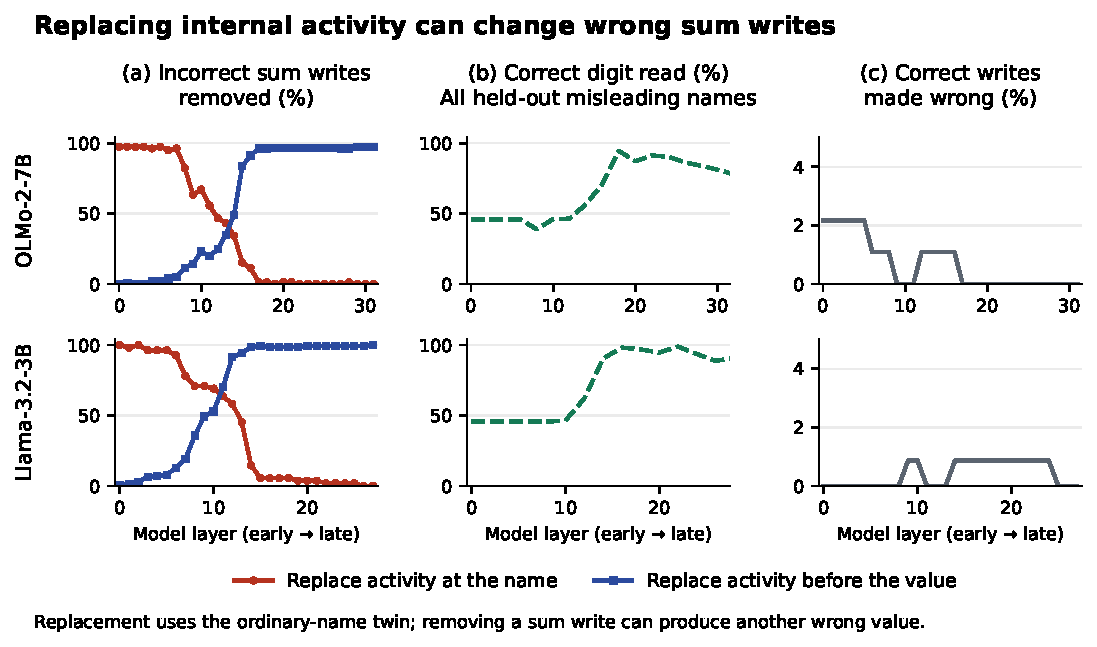
\includegraphics[width=\textwidth]{figures/c_mechanism.pdf}
\caption{\textbf{(a)} Name-error removal. \textbf{(b)} Correct-digit readout.
\textbf{(c)} Damage to correct writes. Patches use ordinary-name twins.}
\label{c-fig:mechanism}
\end{figure*}

We follow \citeauthor{kudo2026faithful}'s 10-class linear-probe recipe, with three seeds and
neutral-only training. Each probe predicts a target digit from one residual-stream position
and layer. Name-identity controls use deterministic random labels keyed on the identifier
\cite{hewitt2019control}. Neutral names and values vary independently, and misleading names
are absent from training. The original implementation reused test programs in training. The reported reruns
replace those scores: they train on \NUM{c-probe-n-train} independent neutral programs and
evaluate \NUM{c-probe-n-test} misleading-name programs, with overlap guards that ignore name
spelling. Table~\ref{c-tab:probe-repeats} reports the name controls alongside digit accuracy.

% Disjoint-probe demonstration repeats
Figure~\ref{c-fig:mechanism}'s probe curves use demonstration set 7. Repeating training and evaluation with sets 11 and 13
gives true-digit accuracies of \NUM{c-probe-olmo7-demo-lo}--\NUM{c-probe-olmo7-demo-hi}\%,
\NUM{c-probe-llama3-demo-lo}--\NUM{c-probe-llama3-demo-hi}\% and
\NUM{c-probe-llama8-demo-lo}--\NUM{c-probe-llama8-demo-hi}\% across the three sets. Each repeat
uses the same independent training programs and three probe seeds; its layer is selected by
that set's neutral accuracy. These repeats assess prompt sensitivity, not a causal role for
the decoded digit. Table~\ref{c-tab:probe-repeats} gives both conditions' readouts and controls.

\begin{table*}[t]
\centering\small
\begin{tabular}{@{}lrrrrrrr@{}}
\toprule
Model & Set & Layer & Neutral & Control & Misleading & Control & Majority \\
\midrule
OLMo-2-7B & 7 & 18 & 99.5 & 100.0 & 94.5 & 33.0 & 45.6 \\
OLMo-2-7B & 11 & 18 & 97.3 & 100.0 & 95.4 & 0.0 & 45.6 \\
OLMo-2-7B & 13 & 18 & 99.8 & 100.0 & 97.4 & 23.4 & 45.6 \\
Llama-3.2-3B & 7 & 24 & 98.8 & 99.7 & 93.7 & 20.0 & 45.6 \\
Llama-3.2-3B & 11 & 20 & 100.0 & 99.8 & 95.4 & 5.0 & 45.6 \\
Llama-3.2-3B & 13 & 28 & 99.4 & 100.0 & 99.9 & 1.9 & 45.6 \\
Llama-3.1-8B & 7 & 16 & 100.0 & 87.8 & 99.9 & 33.0 & 45.6 \\
Llama-3.1-8B & 11 & 20 & 100.0 & 81.6 & 100.0 & 0.1 & 45.6 \\
Llama-3.1-8B & 13 & 20 & 100.0 & 87.2 & 100.0 & 3.0 & 45.6 \\
\bottomrule
\end{tabular}

\caption{Disjoint code probes, three demonstration sets. Neutral and misleading are
true-digit accuracy; each control column gives name-identity accuracy for that condition.
Majority predicts the most frequent digit in training on the misleading test programs.
Rates are percentages, averaged over three probe seeds. Layers are selected by neutral accuracy.}
\label{c-tab:probe-repeats}
\end{table*}

We supply the correct trace token by token when caching probe inputs. The decision position is the \texttt{=} before the
first traced value; later values cannot affect this position under causal attention. Patching
uses only the prompt and this trace prefix. Name patches replace every aligned
occurrence of the identifier; decision patches replace only that writing position. Both use
one layer at a time and include a neutral-for-neutral disruption control
\cite{zhang2024patching}. The alternative-name control is uninformative in the main cell:
every sum-family identifier implies the same sum, so there is no distinct source name-suggested value.
Llama-3.1-8B's affected two-token name lacks aligned neutral twins for the name-site intervention.


\begin{table*}[t]
\centering\small
\begin{tabular}{@{}lrrrrrrr@{}}
\toprule
& \multicolumn{3}{c}{Name tokens} & \multicolumn{4}{c}{Decision token} \\ \cmidrule(lr){2-4}\cmidrule(lr){5-8}
Model & L0 & damage & $<$10\% by & 50\% at & 90\% at & all layers & damage \\
\midrule
OLMo-2-7B & 97\% & 2\% & L17 & L15 & L16 & 97\% & 2\% \\
Llama-3.2-3B & 100\% & 0\% & L15 & L10 & L12 & 100\% & 0\% \\
Llama-3.1-8B & -- & -- & -- & L8 & L9 & 100\% & 0\% \\
\bottomrule
\end{tabular}

\caption{Layers behind Figure~\ref{c-fig:mechanism}. Name tokens: name errors removed by
replacing every token of the name at layer 0, damage to correct instances, and the first
layer after which removal falls below 10\%. Decision token: first layer at which a
single-layer replacement removes 50\% and 90\% of name errors, removal with every layer
replaced, and its damage. Llama-3.1-8B's name errors fall on a two-token name without a
token-aligned twin.}
\label{c-tab:patch}
\end{table*}

\section{Scope checks}
\label{c-app:boundaries}

\paragraph{Operation and scale.} Moving the misleading name to a unary middle step produces
no reliable effect for models above the accuracy floor; the largest excess is
\NUM{c-l6-max-excess} points. CodeLlama-34B's length-to-sum effect is \NUM{c-cell34-len-excess},
while its maximum-to-sum effect is \NUM{c-cell34-max-excess} points
[\NUM{c-cell34-max-lo}, \NUM{c-cell34-max-hi}]. The latter is a reliable positive effect, but its
interval extends beyond the two-point margin. Its small point estimate cannot be reported as
equivalence. The larger-checkpoint result supports the registered maximum-to-sum direction
and reliable-effect criterion, while its magnitude is much smaller than CodeLlama-7B's.

\paragraph{Natural code.} We select \NUM{c-crux-n} CRUXEval functions with length, loop-counter
or maximum assignments, rename the target by AST rewriting to \texttt{v} or \texttt{total},
and verify execution after renaming. Direct and prose accuracy contrasts all have intervals
covering zero on the \NUM{c-crux-used} functions whose renamed target is used downstream.
Their endpoints stay within \NUM{c-crux-direct-bound} and
\NUM{c-crux-prose-bound} points, respectively (Table~\ref{c-tab:crux}). These are bounded results
for those functions and prompts; they do not test the trace that lists values without expressions used in the synthetic
study.
The natural-code functions come from \citet{gu2024cruxeval}.


\begin{table*}[t]
\centering\small
\begin{tabular}{@{}lrrrr@{}}
\toprule
Model & Direct acc. & Direct $\Delta$ & Prose acc. & Prose $\Delta$ \\
\midrule
OLMo-2-7B & 10 & +1.2 [+0.0, +3.6] & 22 & -1.2 [-9.5, +8.3] \\
Llama-3.2-3B & 19 & +1.2 [-2.4, +4.8] & 25 & +3.6 [-3.6, +10.7] \\
Llama-3.1-8B & 22 & -3.6 [-9.5, +2.4] & 40 & +0.0 [-9.5, +9.5] \\
CodeLlama-7B & 18 & +2.4 [+0.0, +6.0] & 13 & +2.4 [-4.8, +9.5] \\
CodeGemma-7B & 18 & +0.0 [-4.8, +4.8] & 22 & +2.4 [-8.3, +13.1] \\
Gemma-3-4B & 15 & -2.4 [-6.0, +0.0] & 45 & +4.8 [-1.2, +11.9] \\
OLMo-2-1B & 16 & -3.6 [-8.3, +0.0] & 3 & +6.0 [+0.0, +11.9] \\
\bottomrule
\end{tabular}

\caption{\NUM{c-crux-n} CRUXEval functions that assign a variable from \texttt{len(\ldots)}
(\NUM{c-crux-kind-len}), a loop counter (\NUM{c-crux-kind-counter}) or \texttt{max(\ldots)}
(\NUM{c-crux-kind-max}), of which \NUM{c-crux-used} use it downstream; each rendered with the
original name, the neutral name \texttt{v}, and the misleading name \texttt{total}. Accuracy
on all neutral renderings, and the paired misleading-minus-neutral difference in points on
the downstream-used subset, with a bootstrap interval over functions.}
\label{c-tab:crux}
\end{table*}


\section{Effect and equivalence checks}
\label{c-app:stats}
Each contrast subtracts the neutral twin's rate for the same digit. We resample matched problems
with demonstration-seed replicates together and use 95\% cluster-bootstrap intervals.
Reliability also requires a consistent sign across all three demonstration sets.

Equivalence applies the $\pm\NUM{c-eq-delta}$-point margin to 90\% intervals from the same
cluster bootstrap (two one-sided 5\% tests), using 2,000 draws. Across \NUM{c-eq-cells} tested contrasts,
\NUM{c-eq-equivalent} intervals lie wholly inside the margin, \NUM{c-eq-witheffect} contrasts have
reliable effects without meeting that bound, and \NUM{c-eq-inconclusive} meet neither criterion.
A small estimate or an interval covering zero does not by itself establish equivalence.

% Generated by scripts/77_followup_tables.py from validated JSON.
\section{Generated-prefix audit and initial readouts}
\label{c-app:round5-errors}
For 2565 of 2565 misleading-name generations, the token prefix through the marker before the first value exactly matches the cached trace. This verifies that the cached state at that marker also precedes the generated value. No target value token is included.
These initial readouts select layers on the full neutral evaluation set; the main text instead uses independent cross-fitted selection (Appendix~\ref{c-app:round6-probes}). We split the generated writes into name-suggested values, correct values and other errors. Table~\ref{c-tab:round5-errors} averages three probe seeds and pools demonstration sets 7, 11 and 13. Intervals resample matched programs with all their demonstration repeats (4,000 draws). These conditional readouts establish available information on observed errors; they do not establish its causal use.
\begin{table*}[t]
\centering\small
\sbox{\roundfivebox}{\begin{tabular}{@{}llrrl@{}}
\toprule
Model & Generated write & Rows & Programs & True-digit accuracy (\%) \\
\midrule
OLMo-2-7B & name error & 503 & 193 & 96.4 [94.8, 97.8] \\
OLMo-2-7B & correct write & 320 & 135 & 96.7 [94.4, 98.5] \\
OLMo-2-7B & other error & 32 & 24 & 77.1 [61.7, 90.5] \\
Llama-3.2-3B & name error & 372 & 169 & 95.7 [93.8, 97.4] \\
Llama-3.2-3B & correct write & 440 & 204 & 98.3 [97.0, 99.3] \\
Llama-3.2-3B & other error & 43 & 29 & 82.2 [71.2, 91.7] \\
Llama-3.1-8B & name error & 106 & 45 & 99.7 [99.0, 100.0] \\
Llama-3.1-8B & correct write & 749 & 261 & 100.0 [100.0, 100.0] \\
Llama-3.1-8B & other error & 0 & 0 & -- \\
\bottomrule
\end{tabular}}
\ifdim\wd\roundfivebox>\textwidth\resizebox{\textwidth}{!}{\usebox{\roundfivebox}}\else\usebox{\roundfivebox}\fi
\caption{Disjoint probes at the verified generated prefix. A dash denotes an empty stratum. The denominator is observed writes within each stratum, not independent demonstration repeats.}
\label{c-tab:round5-errors}
\end{table*}
\section{Sensitivity to identifier meanings}
\label{c-app:round5-identifiers}
None of the three main-cell names (\texttt{total}, \texttt{sum\_all}, \texttt{acc}) meets the originally planned 80\% panel gate. Its filtered estimate is therefore unavailable, rather than zero.
Table~\ref{c-tab:round5-identifiers} retains the full-data estimate and reports each name and each model's own meaning gate. Gates use the original saved meaning checks. Intervals cluster matched programs across the three demonstration sets. This exploratory sensitivity does not replace the planned panel gate or remove the deviation from it.
\begin{table*}[t]
\centering\small
\sbox{\roundfivebox}{\begin{tabular}{@{}llllll@{}}
\toprule
Model & All & Model gate & \texttt{total} & \texttt{sum\_all} & \texttt{acc} \\
\midrule
Gemma-3-4B & 0.0 [0.0, 0.0] & -- & 0.0 [0.0, 0.0] & 0.0 [0.0, 0.0] & 0.0 [0.0, 0.0] \\
CodeGemma-7B & 0.1 [0.0, 0.4] & 0.1 [0.0, 0.4] & 0.0 [0.0, 0.0] & 0.3 [0.0, 1.0] & 0.0 [0.0, 0.0] \\
Llama-3.1-8B & 12.4 [8.9, 16.0] & 12.4 [8.9, 16.0] & 0.0 [0.0, 0.0] & 34.0 [26.0, 42.3] & 0.0 [0.0, 0.0] \\
OLMo-2-1B & 3.7 [2.2, 5.5] & 5.0 [1.8, 8.9] & 5.0 [1.8, 8.9] & 5.8 [2.6, 9.3] & 0.0 [0.0, 0.0] \\
OLMo-2-7B & 58.4 [53.1, 63.4] & 59.3 [52.7, 65.8] & 56.4 [47.9, 64.9] & 96.2 [93.9, 98.1] & 15.3 [9.6, 21.8] \\
CodeLlama-7B & 3.7 [2.1, 5.5] & 3.7 [2.1, 5.5] & 1.8 [0.4, 3.2] & 8.7 [4.5, 13.1] & 0.0 [0.0, 0.0] \\
Llama-3.2-3B & 43.4 [38.5, 48.0] & 43.4 [38.5, 48.0] & 30.1 [23.8, 36.9] & 76.3 [70.2, 82.4] & 18.4 [11.9, 25.7] \\
\bottomrule
\end{tabular}}
\ifdim\wd\roundfivebox>\textwidth\resizebox{\textwidth}{!}{\usebox{\roundfivebox}}\else\usebox{\roundfivebox}\fi
\caption{Excess name errors in percentage points [95\% interval], level 5 length-to-sum. Empty subsets are shown as dashes. The saved JSON also reports each demonstration set and the all-three-sets sign rule.}
\label{c-tab:round5-identifiers}
\end{table*}
\section{Length and numeric elaboration controls}
\label{c-app:round5-formats}
We add neutral annotations to each demonstrated value, matching the expression demonstrations' token counts, and separately add valid numeric elaborations of the form \texttt{name = value + 0 = value}. The test program and \texttt{Trace:} prefix are unchanged. Greedy decoding uses the same 285 misleading programs and neutral twins for each format. Table~\ref{c-tab:round5-formats} pools three demonstration sets; changes relative to the original trace and expression trace are paired on the same programs.
The length-matched annotation controls retain much larger excess than expression demonstrations in both models. Numeric elaboration reduces excess relative to the original trace but leaves a larger effect than source expressions. Token count alone does not reproduce the expression benefit, and adding valid arithmetic accounts for part of it; these two contrasts do not isolate a single mechanism.
\begin{table*}[t]
\centering\small
\sbox{\roundfivebox}{\begin{tabular}{@{}lllll@{}}
\toprule
Model & Format & Excess & Change vs trace & Change vs expression \\
\midrule
OLMo-2-7B & neutral annotation & 56.6 [51.3, 61.6] & -1.8 [-3.4, -0.1] & 53.2 [48.1, 58.2] \\
OLMo-2-7B & numeric elaboration & 41.3 [36.4, 46.0] & -17.1 [-21.1, -12.9] & 37.9 [33.2, 42.5] \\
Llama-3.2-3B & neutral annotation & 49.6 [44.7, 54.3] & 6.2 [4.1, 8.4] & 49.2 [44.3, 53.9] \\
Llama-3.2-3B & numeric elaboration & 14.9 [12.0, 17.8] & -28.5 [-32.7, -24.3] & 14.5 [11.7, 17.4] \\
\bottomrule
\end{tabular}}
\ifdim\wd\roundfivebox>\textwidth\resizebox{\textwidth}{!}{\usebox{\roundfivebox}}\else\usebox{\roundfivebox}\fi
\caption{Excess name errors and paired changes in percentage points [95\% interval]. Bootstrap clusters keep all demonstration repeats for each matched program together. These controls assess length and numeric elaboration; they do not by themselves establish how expressions change generation.}
\label{c-tab:round5-formats}
\end{table*}

% Generated from validated round-six summaries.
\section{Independent probe layer selection}
\label{c-app:round6-probes}
The main-text error readouts use five-fold cross-fitting. A fixed SHA256 hash assigns canonical program computations to folds, keeping renamed versions and demonstration repeats together. For each held-out fold, we select the layer with the highest neutral accuracy on the other four folds, averaging three probe seeds and breaking ties toward the lowest layer. Neither the held-out neutral labels nor its misleading writes enter that choice. Probe training remains disjoint from every evaluation computation.
Each program is scored only with its held-out fold's layer. The generated-prefix audit from Appendix~\ref{c-app:round5-errors} still applies. Table~\ref{c-tab:round6-probes} reports the conditional write strata and paired changes from the earlier full-neutral selection. Intervals use 4,000 canonical-program bootstrap draws, keeping demonstration repeats together. They condition on the fixed fold selectors and do not refit layer selection inside each bootstrap. Name controls and the full layer curves remain descriptive measurements in Appendix~\ref{c-app:probes}.
\begin{table*}[t]
\centering\small
\sbox{\roundsixbox}{\begin{tabular}{@{}llrrll@{}}
\toprule
Model & Write & Rows & Computations & Accuracy (\%) & Change (points) \\
\midrule
OLMo-2-7B & name error & 503 & 193 & 96.4 [94.9, 97.9] & 0.0 [0.0, 0.0] \\
OLMo-2-7B & correct write & 320 & 135 & 96.7 [94.4, 98.4] & 0.0 [0.0, 0.0] \\
OLMo-2-7B & other error & 32 & 24 & 77.1 [61.6, 90.6] & 0.0 [0.0, 0.0] \\
Llama-3.2-3B & name error & 372 & 169 & 95.5 [93.6, 97.3] & -0.2 [-0.9, 0.4] \\
Llama-3.2-3B & correct write & 440 & 204 & 98.0 [96.6, 99.1] & -0.3 [-0.8, 0.0] \\
Llama-3.2-3B & other error & 43 & 29 & 82.2 [71.1, 91.7] & 0.0 [0.0, 0.0] \\
Llama-3.1-8B & name error & 106 & 45 & 99.7 [99.0, 100.0] & 0.0 [0.0, 0.0] \\
Llama-3.1-8B & correct write & 749 & 261 & 100.0 [99.9, 100.0] & -0.0 [-0.1, 0.0] \\
Llama-3.1-8B & other error & 0 & 0 & -- & -- \\
\bottomrule
\end{tabular}}
\ifdim\wd\roundsixbox>\textwidth\resizebox{\textwidth}{!}{\usebox{\roundsixbox}}\else\usebox{\roundsixbox}\fi
\caption{True-digit readouts with independent layer selection. Changes compare the same observed writes with the earlier full-neutral layer choice. A dash denotes an empty stratum. These readouts establish decodability, not causal use.}
\label{c-tab:round6-probes}
\end{table*}
\section{Independent replication with screened names}
\label{c-app:round6-identifiers}
We fix \NUM{c-r6-screen-n} fresh sum-family candidates before scoring them with the original candidate-continuation meaning check (Appendix~\ref{c-app:gate}). The panel is the same seven models used for that gate. A name qualifies when sum is the highest-scoring continuation in at least 80\% of the panel; ties follow the original scoring order. Two additional function-name contexts and neutral names are diagnostic and do not affect selection. Of the candidates, \NUM{c-r6-screen-passed} qualify. We freeze the first \NUM{c-r6-name-n} qualifying names in the fixed order: \NUM{c-r6-name-list}. No trace outcomes enter selection.
The replication uses \NUM{c-r6-program-n} new length-computed programs. Their canonical computations are unique and absent from the original level-5 training and test corpus and all three demonstration sets. True and name-suggested values are checked by execution and retain the original value-exclusion rules. Every selected name is crossed with every program; its neutral twin differs only in the target identifier. The three affected models and the prespecified CodeGemma-7B control use the same programs and demonstration sets 7, 11 and 13 under trace and expression demonstrations.
Table~\ref{c-tab:round6-replication} pools names and demonstration sets, clustering all repeats of each computation in 4,000 bootstrap draws. Table~\ref{c-tab:round6-replication-names} reports each identifier. The format contrast replicates on independently selected names, but names and programs differ from the original experiment, so differences in effect magnitude across the two samples are descriptive. This exploratory replication does not retroactively repair the original selection-rule deviation. Probes and patches concern the original identifiers, not these new names.
\begin{table*}[t]
\centering\small
\sbox{\roundsixbox}{\begin{tabular}{@{}lccc@{}}
\toprule
Candidate & Sum agreement & Qualifies & Selected \\
\midrule
\texttt{sum\_of\_values} & 6/7 & yes & yes \\
\texttt{sum\_of\_items} & 7/7 & yes & yes \\
\texttt{sum\_of\_elements} & 7/7 & yes & yes \\
\texttt{sum\_of\_xs} & 7/7 & yes & no \\
\texttt{sum\_of\_list} & 6/7 & yes & no \\
\texttt{list\_sum} & 6/7 & yes & no \\
\texttt{input\_sum} & 6/7 & yes & no \\
\texttt{items\_sum} & 6/7 & yes & no \\
\texttt{elements\_sum} & 5/7 & no & no \\
\texttt{sum\_values} & 5/7 & no & no \\
\texttt{sum\_result} & 6/7 & yes & no \\
\texttt{sum\_total} & 6/7 & yes & no \\
\texttt{total\_sum} & 6/7 & yes & no \\
\texttt{xs\_sum} & 7/7 & yes & no \\
\texttt{sum\_xs} & 7/7 & yes & no \\
\texttt{summation} & 6/7 & yes & no \\
\bottomrule
\end{tabular}}
\ifdim\wd\roundsixbox>\textwidth\resizebox{\textwidth}{!}{\usebox{\roundsixbox}}\else\usebox{\roundsixbox}\fi
\caption{The entire fixed candidate list, in selection order. Qualification uses the original canonical meaning prompt. Selection retains the first three qualifying candidates without consulting behavior.}
\label{c-tab:round6-screen}
\end{table*}
\begin{table*}[t]
\centering\small
\sbox{\roundsixbox}{\begin{tabular}{@{}llll@{}}
\toprule
Model & Trace excess & Expression excess & Expression minus trace \\
\midrule
OLMo-2-7B & 91.1 [88.4, 93.6] & 0.8 [0.3, 1.3] & -90.3 [-92.9, -87.6] \\
Llama-3.2-3B & 61.5 [56.1, 66.9] & 0.0 [0.0, 0.0] & -61.5 [-66.9, -56.1] \\
Llama-3.1-8B & 16.7 [12.8, 20.8] & 0.0 [0.0, 0.0] & -16.7 [-20.8, -12.8] \\
CodeGemma-7B & 0.0 [0.0, 0.0] & 0.0 [0.0, 0.0] & 0.0 [0.0, 0.0] \\
\bottomrule
\end{tabular}}
\ifdim\wd\roundsixbox>\textwidth\resizebox{\textwidth}{!}{\usebox{\roundsixbox}}\else\usebox{\roundsixbox}\fi
\caption{Independent screened-name replication: excess name errors and paired format changes in percentage points [95\% interval]. All selected identifiers and three demonstration sets are pooled over 200 fresh computations. A zero bootstrap interval records no observed paired name errors; it is not a population-level absence or equivalence claim.}
\label{c-tab:round6-replication}
\end{table*}
\begin{table*}[t]
\centering\small
\sbox{\roundsixbox}{\begin{tabular}{@{}llll@{}}
\toprule
Model & Identifier & Trace excess & Expression excess \\
\midrule
OLMo-2-7B & \texttt{sum\_of\_values} & 91.7 [88.8, 94.3] & 0.2 [0.0, 0.5] \\
OLMo-2-7B & \texttt{sum\_of\_items} & 89.2 [86.0, 92.0] & 2.0 [0.8, 3.3] \\
OLMo-2-7B & \texttt{sum\_of\_elements} & 92.5 [89.8, 94.8] & 0.2 [0.0, 0.5] \\
Llama-3.2-3B & \texttt{sum\_of\_values} & 61.7 [56.0, 67.3] & 0.0 [0.0, 0.0] \\
Llama-3.2-3B & \texttt{sum\_of\_items} & 55.5 [50.0, 61.3] & 0.0 [0.0, 0.0] \\
Llama-3.2-3B & \texttt{sum\_of\_elements} & 67.3 [61.7, 73.0] & 0.0 [0.0, 0.0] \\
Llama-3.1-8B & \texttt{sum\_of\_values} & 12.8 [9.3, 16.7] & 0.0 [0.0, 0.0] \\
Llama-3.1-8B & \texttt{sum\_of\_items} & 22.8 [18.0, 27.7] & 0.0 [0.0, 0.0] \\
Llama-3.1-8B & \texttt{sum\_of\_elements} & 14.5 [10.5, 18.7] & 0.0 [0.0, 0.0] \\
CodeGemma-7B & \texttt{sum\_of\_values} & 0.0 [0.0, 0.0] & 0.0 [0.0, 0.0] \\
CodeGemma-7B & \texttt{sum\_of\_items} & 0.0 [0.0, 0.0] & 0.0 [0.0, 0.0] \\
CodeGemma-7B & \texttt{sum\_of\_elements} & 0.0 [0.0, 0.0] & 0.0 [0.0, 0.0] \\
\bottomrule
\end{tabular}}
\ifdim\wd\roundsixbox>\textwidth\resizebox{\textwidth}{!}{\usebox{\roundsixbox}}\else\usebox{\roundsixbox}\fi
\caption{Per-identifier replication, pooling the same three demonstration sets. Effects are percentage points [95\% canonical-program bootstrap interval]. All affected-model trace means are positive in every demonstration set; per-set estimates are retained in the saved summary.}
\label{c-tab:round6-replication-names}
\end{table*}

\section{Prompt-end versus pre-write readouts}
\label{c-app:prompt-comparison}
We fit separate probes at the final token of the complete prompt ending in \texttt{Trace:}, before generating any trace token. Tokenization of this prefix is checked against the original continuation. Training computations, demonstration sets, SGD recipe and seeds match the pre-write probes. Each position selects its layer independently using the same five canonical-computation folds and other folds' neutral labels. Outcome strata and generated-prefix eligibility are frozen from the previous audit. Intervals use 4,000 paired canonical-computation bootstrap draws and condition on the fixed selectors.
\begin{table*}[t]
\centering\small
\sbox{\centralbox}{\begin{tabular}{@{}llrrrrr@{}}
\toprule
Model & Write & Rows / computations & Prompt & Before write & Change & Name ID \\
\midrule
OLMo-2-7B & sum write & 503 / 193 & 38.4 [32.9, 43.9] & 96.4 [94.9, 97.9] & +58.1 [+52.6, +63.4] & 12.7 [9.8, 15.9] \\
OLMo-2-7B & correct write & 320 / 135 & 35.2 [27.7, 43.1] & 96.7 [94.4, 98.4] & +61.5 [+53.3, +69.3] & 20.8 [15.5, 26.3] \\
OLMo-2-7B & other error & 32 / 24 & 76.0 [58.1, 90.2] & 77.1 [61.6, 90.6] & +1.0 [-19.6, +22.6] & 26.0 [12.6, 41.1] \\
Llama-3.2-3B & sum write & 372 / 169 & 26.4 [22.4, 30.8] & 95.5 [93.6, 97.3] & +69.1 [+64.5, +73.4] & 0.7 [0.1, 1.6] \\
Llama-3.2-3B & correct write & 440 / 204 & 37.9 [32.1, 43.7] & 98.0 [96.6, 99.1] & +60.1 [+54.4, +65.8] & 3.6 [1.8, 5.7] \\
Llama-3.2-3B & other error & 43 / 29 & 20.9 [11.7, 31.7] & 82.2 [71.1, 91.7] & +61.2 [+46.8, +73.8] & 2.3 [0.0, 6.1] \\
Llama-3.1-8B & sum write & 106 / 45 & 56.0 [47.4, 64.2] & 99.7 [99.0, 100.0] & +43.7 [+35.4, +52.4] & 0.0 [0.0, 0.0] \\
Llama-3.1-8B & correct write & 749 / 261 & 49.9 [45.7, 54.1] & 100.0 [99.9, 100.0] & +50.1 [+45.8, +54.3] & 0.0 [0.0, 0.0] \\
Llama-3.1-8B & other error & 0 / 0 & -- & -- & -- & -- \\
\bottomrule
\end{tabular}}
\ifdim\wd\centralbox>\textwidth\resizebox{\textwidth}{!}{\usebox{\centralbox}}\else\usebox{\centralbox}\fi
\caption{Paired true-digit accuracies and prompt-position name-identity controls (\%) [95\% interval]. Change is pre-write minus prompt accuracy in points.}
\label{c-tab:prompt-comparison}
\end{table*}

\section{Reproducibility and model terms}
\label{c-app:reproducibility}

The main panel contains seven instruction-tuned checkpoints, with CodeLlama-34B as a
scale check. We use CodeLlama \citep{roziere2023codellama}, CodeGemma
\citep{codegemmateam2024codegemma}, Llama~3 \citep{grattafiori2024llama3}, Gemma~3
\citep{gemmateam2025gemma3} and OLMo~2 \citep{olmo2024olmo2,walsh2025olmo2}.
The model identifiers are \texttt{codellama/CodeLlama-7b-Instruct-hf} and its 34b variant,
\texttt{google/codegemma-7b-it}, \texttt{meta-llama/Llama-3.2-3B-Instruct},
\texttt{meta-llama/Llama-3.1-8B-Instruct}, \texttt{google/gemma-3-4b-it},
\texttt{allenai/OLMo-2-0425-1B-Instruct} and \texttt{allenai/OLMo-2-1124-7B-Instruct}.
These use the Llama~2/CodeLlama, Llama~3.1 or 3.2 Community Licenses, Gemma Terms of Use,
and Apache~2.0, respectively. The study uses their released weights for research inference
and does not redistribute weights. CRUXEval uses the MIT license.

Synthetic data consist of digits, generated identifiers and short Python functions,
without personal records or human annotations. Each tested level has 1,000 matched
problems per target. Main behavior uses three sets of three demonstrations with seeds
7, 11 and 13; programs and demonstration identities remain fixed across compared formats.
Greedy decoding uses the full vocabulary. Parsers retain failed outputs in denominators;
trace-error measurements use the first assignment, while final-answer accuracy scores
the reported return value. Probe training and testing are disjoint in arithmetic computation,
ignoring identifier spelling. The independent-name replication uses separate screened
names and 200 new computations, as described in Appendix~\ref{c-app:round6-identifiers}.

Probes use full-batch SGD with learning rate $10^{-3}$ for 10,000 epochs and seeds 0, 1 and 2.
Five-fold layer selection is disjoint in computation; bootstrap intervals condition on
those selectors. These are linear-predictor fits, not language-model training.
Combined recorded allocations across the arithmetic and code experiments total
\NUM{c-compute-shared-gpuh} GPU-hours on NVIDIA A30, H100 and H200 GPUs, an upper bound
including idle and shared workers. Software is PyTorch~2.11.0 (CUDA~12.9)
\citep{paszke2019pytorch}, Transformers~5.14.1 \citep{wolf2020transformers},
NumPy~2.3.5 and scikit-learn~1.9.1 \citep{pedregosa2011sklearn}.



\begin{table*}[t]
\centering\small
% Generated by scripts/83_main_evidence.py from validated summaries.
\sbox{\centralbox}{\begin{tabular}{@{}lrrrr@{}}
\toprule
Model & \shortstack{Extra sum writes\\(points)} & \shortstack{Correct digit (\%)\\Before trace} & \shortstack{Correct digit (\%)\\Before wrong value} & \shortstack{Wrong writes\\(unique programs)} \\
\midrule
OLMo-2-7B & +58.4 & 38.4 [32.9, 43.9] & 96.4 [94.9, 97.9] & 503 (193) \\
Llama-3.2-3B & +43.4 & 26.4 [22.4, 30.8] & 95.5 [93.6, 97.3] & 372 (169) \\
Llama-3.1-8B & +12.4 & 56.0 [47.4, 64.2] & 99.7 [99.0, 100.0] & 106 (45) \\
\bottomrule
\end{tabular}}
\ifdim\wd\centralbox>\textwidth\resizebox{\textwidth}{!}{\usebox{\centralbox}}\else\usebox{\centralbox}\fi

\caption{Code behavior and error-conditioned readouts [95\% interval]. Counts distinguish writes from computations.}
\label{c-tab:central}
\end{table*}

\section{Correctness on the matched code format cohort}
\label{app:format-correctness}
We score the first written value and final answer on the same 285 original length-to-sum programs and their ordinary-name twins, under values-only and expression-and-value examples. Each format has 855 paired observations over three demonstration sets. Parse failures count as incorrect. Intervals use 4,000 bootstrap draws over matched program IDs, keeping all demonstration repeats and both names together. The format changes are paired on those same IDs. These are overall correctness rates within the specified cohort, rather than the larger task pool. Zero-width intervals record this sample, not certainty about population rates.
\begin{table*}[t]\centering\small
\begin{tabular}{@{}lllrr@{}}
\toprule
Model & Examples & Names & Correct first value (\%) & Correct final answer (\%) \\
\midrule
OLMo-2-7B-I & Values only & Ordinary & \NUM{j-format-olmo7-values-ordinary-first-mean} [\NUM{j-format-olmo7-values-ordinary-first-lo}, \NUM{j-format-olmo7-values-ordinary-first-hi}] & \NUM{j-format-olmo7-values-ordinary-final-mean} [\NUM{j-format-olmo7-values-ordinary-final-lo}, \NUM{j-format-olmo7-values-ordinary-final-hi}] \\
OLMo-2-7B-I & Values only & Misleading & \NUM{j-format-olmo7-values-misleading-first-mean} [\NUM{j-format-olmo7-values-misleading-first-lo}, \NUM{j-format-olmo7-values-misleading-first-hi}] & \NUM{j-format-olmo7-values-misleading-final-mean} [\NUM{j-format-olmo7-values-misleading-final-lo}, \NUM{j-format-olmo7-values-misleading-final-hi}] \\
OLMo-2-7B-I & Expression + value & Ordinary & \NUM{j-format-olmo7-expression-ordinary-first-mean} [\NUM{j-format-olmo7-expression-ordinary-first-lo}, \NUM{j-format-olmo7-expression-ordinary-first-hi}] & \NUM{j-format-olmo7-expression-ordinary-final-mean} [\NUM{j-format-olmo7-expression-ordinary-final-lo}, \NUM{j-format-olmo7-expression-ordinary-final-hi}] \\
OLMo-2-7B-I & Expression + value & Misleading & \NUM{j-format-olmo7-expression-misleading-first-mean} [\NUM{j-format-olmo7-expression-misleading-first-lo}, \NUM{j-format-olmo7-expression-misleading-first-hi}] & \NUM{j-format-olmo7-expression-misleading-final-mean} [\NUM{j-format-olmo7-expression-misleading-final-lo}, \NUM{j-format-olmo7-expression-misleading-final-hi}] \\
\addlinespace
Llama-3.2-3B-I & Values only & Ordinary & \NUM{j-format-llama3-values-ordinary-first-mean} [\NUM{j-format-llama3-values-ordinary-first-lo}, \NUM{j-format-llama3-values-ordinary-first-hi}] & \NUM{j-format-llama3-values-ordinary-final-mean} [\NUM{j-format-llama3-values-ordinary-final-lo}, \NUM{j-format-llama3-values-ordinary-final-hi}] \\
Llama-3.2-3B-I & Values only & Misleading & \NUM{j-format-llama3-values-misleading-first-mean} [\NUM{j-format-llama3-values-misleading-first-lo}, \NUM{j-format-llama3-values-misleading-first-hi}] & \NUM{j-format-llama3-values-misleading-final-mean} [\NUM{j-format-llama3-values-misleading-final-lo}, \NUM{j-format-llama3-values-misleading-final-hi}] \\
Llama-3.2-3B-I & Expression + value & Ordinary & \NUM{j-format-llama3-expression-ordinary-first-mean} [\NUM{j-format-llama3-expression-ordinary-first-lo}, \NUM{j-format-llama3-expression-ordinary-first-hi}] & \NUM{j-format-llama3-expression-ordinary-final-mean} [\NUM{j-format-llama3-expression-ordinary-final-lo}, \NUM{j-format-llama3-expression-ordinary-final-hi}] \\
Llama-3.2-3B-I & Expression + value & Misleading & \NUM{j-format-llama3-expression-misleading-first-mean} [\NUM{j-format-llama3-expression-misleading-first-lo}, \NUM{j-format-llama3-expression-misleading-first-hi}] & \NUM{j-format-llama3-expression-misleading-final-mean} [\NUM{j-format-llama3-expression-misleading-final-lo}, \NUM{j-format-llama3-expression-misleading-final-hi}] \\
\addlinespace
Llama-3.1-8B-I & Values only & Ordinary & \NUM{j-format-llama8-values-ordinary-first-mean} [\NUM{j-format-llama8-values-ordinary-first-lo}, \NUM{j-format-llama8-values-ordinary-first-hi}] & \NUM{j-format-llama8-values-ordinary-final-mean} [\NUM{j-format-llama8-values-ordinary-final-lo}, \NUM{j-format-llama8-values-ordinary-final-hi}] \\
Llama-3.1-8B-I & Values only & Misleading & \NUM{j-format-llama8-values-misleading-first-mean} [\NUM{j-format-llama8-values-misleading-first-lo}, \NUM{j-format-llama8-values-misleading-first-hi}] & \NUM{j-format-llama8-values-misleading-final-mean} [\NUM{j-format-llama8-values-misleading-final-lo}, \NUM{j-format-llama8-values-misleading-final-hi}] \\
Llama-3.1-8B-I & Expression + value & Ordinary & \NUM{j-format-llama8-expression-ordinary-first-mean} [\NUM{j-format-llama8-expression-ordinary-first-lo}, \NUM{j-format-llama8-expression-ordinary-first-hi}] & \NUM{j-format-llama8-expression-ordinary-final-mean} [\NUM{j-format-llama8-expression-ordinary-final-lo}, \NUM{j-format-llama8-expression-ordinary-final-hi}] \\
Llama-3.1-8B-I & Expression + value & Misleading & \NUM{j-format-llama8-expression-misleading-first-mean} [\NUM{j-format-llama8-expression-misleading-first-lo}, \NUM{j-format-llama8-expression-misleading-first-hi}] & \NUM{j-format-llama8-expression-misleading-final-mean} [\NUM{j-format-llama8-expression-misleading-final-lo}, \NUM{j-format-llama8-expression-misleading-final-hi}] \\
\addlinespace
\midrule
\multicolumn{5}{l}{Expression minus values-only correctness (percentage points)} \\
\midrule
OLMo-2-7B-I & Paired change & Ordinary & \NUM{j-format-olmo7-change-ordinary-first-mean} [\NUM{j-format-olmo7-change-ordinary-first-lo}, \NUM{j-format-olmo7-change-ordinary-first-hi}] & \NUM{j-format-olmo7-change-ordinary-final-mean} [\NUM{j-format-olmo7-change-ordinary-final-lo}, \NUM{j-format-olmo7-change-ordinary-final-hi}] \\
OLMo-2-7B-I & Paired change & Misleading & \NUM{j-format-olmo7-change-misleading-first-mean} [\NUM{j-format-olmo7-change-misleading-first-lo}, \NUM{j-format-olmo7-change-misleading-first-hi}] & \NUM{j-format-olmo7-change-misleading-final-mean} [\NUM{j-format-olmo7-change-misleading-final-lo}, \NUM{j-format-olmo7-change-misleading-final-hi}] \\
Llama-3.2-3B-I & Paired change & Ordinary & \NUM{j-format-llama3-change-ordinary-first-mean} [\NUM{j-format-llama3-change-ordinary-first-lo}, \NUM{j-format-llama3-change-ordinary-first-hi}] & \NUM{j-format-llama3-change-ordinary-final-mean} [\NUM{j-format-llama3-change-ordinary-final-lo}, \NUM{j-format-llama3-change-ordinary-final-hi}] \\
Llama-3.2-3B-I & Paired change & Misleading & \NUM{j-format-llama3-change-misleading-first-mean} [\NUM{j-format-llama3-change-misleading-first-lo}, \NUM{j-format-llama3-change-misleading-first-hi}] & \NUM{j-format-llama3-change-misleading-final-mean} [\NUM{j-format-llama3-change-misleading-final-lo}, \NUM{j-format-llama3-change-misleading-final-hi}] \\
Llama-3.1-8B-I & Paired change & Ordinary & \NUM{j-format-llama8-change-ordinary-first-mean} [\NUM{j-format-llama8-change-ordinary-first-lo}, \NUM{j-format-llama8-change-ordinary-first-hi}] & \NUM{j-format-llama8-change-ordinary-final-mean} [\NUM{j-format-llama8-change-ordinary-final-lo}, \NUM{j-format-llama8-change-ordinary-final-hi}] \\
Llama-3.1-8B-I & Paired change & Misleading & \NUM{j-format-llama8-change-misleading-first-mean} [\NUM{j-format-llama8-change-misleading-first-lo}, \NUM{j-format-llama8-change-misleading-first-hi}] & \NUM{j-format-llama8-change-misleading-final-mean} [\NUM{j-format-llama8-change-misleading-final-lo}, \NUM{j-format-llama8-change-misleading-final-hi}] \\
\bottomrule
\end{tabular}

\caption{Matched-code correctness and paired format changes (95\% intervals).}
\label{tab:format-correctness}
\end{table*}
